\section{Design}\label{Design}

SplitTCP design

Linux integration Design goals
 -No modifications to fast path
 -Edge case operations can take as long as necessary

Compromises
 -Fast path doesn't forward ARP packets after SYN
	*Handle ARPs manually instead of using real ARPs
 -Seperate sequence numbers for Linux and Splittcp
    *Because Splittcp initializes fast path state on receiving SYN, three options:
		1) Add artificial delay or add synchronization with tap thread to use Linux seq
		2) Modify fast path to identify Linux seq and update state
		3) keep separate sequence numbers for Linux and Splittcp
		(we do 3 but might want to switch to 1 eventually)
 -Generate ACK packets in slow path
	*Fast path doesn't forward ACK packets to slow path
	*Manually generate ACK packets

\begin{figure}
\centering
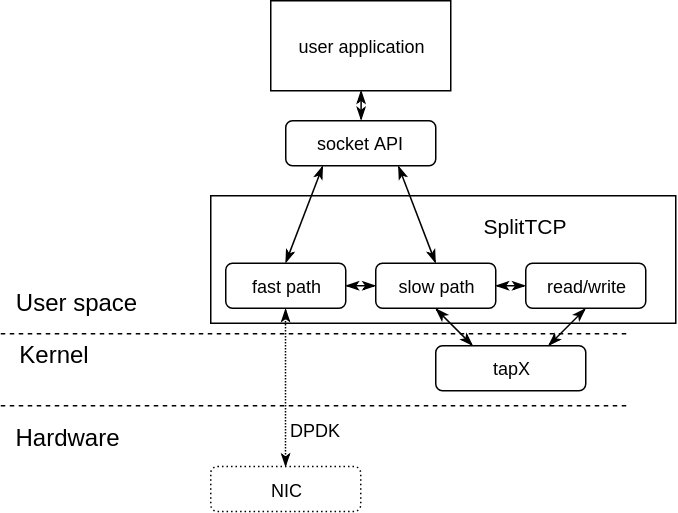
\includegraphics[width=0.7\columnwidth]{figures/splittcp.png}
\caption{Design of TAS with kernel integration. TAS now replicates all slow path operations to the kernel, checks what
it did by reading raw packets from the TAP device and mimics its decisions.}
\label{fig:splittcp_tap}
\end{figure}